% PySyzygos math slides: workflow, conventions, notation, astrometry and the exact solver (input file).
% Included by docs/math/pysyzygos_math.tex (public) and the talk. Slide IDs (\slideid) and formula numbers
% (\tag, \eqtag) are cited in the code as "# Math: <ID>.<n>"; run docs/math/check_xref.py after changes.

% workflow as in the code: data -> screen.py (linear pm, RK4 orbits) -> pick / prescreen -> search.py -> hit
\begin{frame}{Workflow: from catalogs to a hit}
  \centering\vspace*{-2ex}
  \begin{tikzpicture}[
      node distance=0.3cm,
      box/.style={draw=syzblue, fill=syzblue, text=white, rounded corners=3pt, minimum height=1.4cm,
                   text width=2.2cm, align=center, font=\small\bfseries},
      hit/.style={box, draw=syzaccent, fill=syzaccent},
      note/.style={text width=2.45cm, align=left, font=\scriptsize, text=black!75, anchor=north,
                   execute at begin node={\hyphenpenalty=10000\exhyphenpenalty=10000}},
      arr/.style={-Stealth, very thick, syzaccent}]
    \node[box] (data) {Star +\\asteroid data};
    \node[box, right=of data] (corr) {Basic\\corrections};
    \node[box, right=of corr] (pre)  {Target\\pre-screening};
    \node[box, right=of pre]  (srch) {Search};
    \node[hit,  right=of srch] (hit)  {Hit};
    \foreach \a/\b in {data/corr, corr/pre, pre/srch, srch/hit} \draw[arr] (\a) -- (\b);

    \node[note] at ([yshift=-0.35cm]data.south) {%
      Gaia DR3, local copy (G $\le$ 16 / 18, supplement)\\[0.4ex]
      SBDB orbital elements of all asteroids\\[0.4ex]
      JPL Horizons orbits of the targets};
    \node[note] at ([yshift=-0.35cm]corr.south) {%
      Stars: proper motion to the date (linear)\\[0.4ex]
      Asteroids: own RK4 orbits, Sun + planets ($\approx$\,2\,km)};
    \node[note] at ([yshift=-0.35cm]pre.south) {%
      Pick / pre-screens: all asteroids against the bright stars\\[0.4ex]
      Site, altitudes, Sun, drop\\[0.4ex]
      $\to$ target list};
    \node[note] at ([yshift=-0.35cm]srch.south) {%
      Per target: Horizons orbit, Gaia corridor scan\\[0.4ex]
      Full astrometry (space motion, parallax, deflection)\\[0.4ex]
      Exact solver: closest approach};
    \node[note] at ([yshift=-0.35cm]hit.south) {%
      $d_{\min} < r_{\max} + \text{reach}$\\[0.4ex]
      Observable, \mbox{$\Delta m \ge 0.1$}\\[0.4ex]
      $\to$ report, map, KML, favorites};
  \end{tikzpicture}
\end{frame}

% ------------------------------------------------------------------------------------------------- the need for speed
\subsection{Finding candidates fast}
% numbers: a pick + search of one site, 2026-10-20 + 20 days (step tables of the runs, the user's Mac, 1.3.3)
\begin{frame}{The need for speed}\slideid{SP}
  \small
  Every asteroid against every star, for one site: far too much for exact solving. Each stage keeps a superset and
  hands it to a more exact (and more expensive) one:\\[0.6ex]
  \centering
  \begin{tikzpicture}[font=\footnotesize, every node/.style={inner sep=2pt}]
    \foreach \w/\y/\n/\c in {4.6/0/{464{,}740 asteroids}/syzblue!85, 3.9/-0.6/{12{,}808 asteroids}/syzblue!70,
                            3.2/-1.2/{1{,}195 events}/syzblue!55, 2.5/-1.8/{400 targets}/syzaccent!70,
                            1.8/-2.4/{430 hits}/syzaccent}
      \node[fill=\c, text=white, minimum width=\w cm, minimum height=0.5cm, rounded corners=2pt] at (0,\y) {\n};
    \foreach \y/\t in {0/{all of JPL SBDB with $H < 17$},
                       -0.6/{world pre-screen, site test: 17.7\,s {\scriptsize(built once for 40 days: 7.8\,h\footnotemark)}},
                       -1.2/{pick: own orbits, corridor scan, site solve: 16.6\,s},
                       -1.8/{the best events of the pick},
                       -2.4/{search: 3{,}035 candidates, 1{,}301 exact solves: 70\,s}}
      \node[anchor=west, text=black!75] at (2.6,\y) {\t};
  \end{tikzpicture}\\[0.6ex]
  \raggedright
  {\scriptsize One site, 20 days, stars to $G = 15$ (2026-10-20), on the author's Mac. Only the last stage uses
  JPL Horizons orbits, the full astrometry (ST) and the exact solver (IN--OV).}
  \footnotetext{\scriptsize World pre-screen 2026-10-01 + 40 days, G $\le$ 16: 464{,}740 asteroids screened,
    19.3 million events of 461{,}867 asteroids, 1.5 GB; built in 28{,}152\,s on an Intel Core i7-6700K
    (4 cores / 8 threads, 4.0\,GHz), 32\,GB RAM, Linux, 4 worker processes.}
\end{frame}

% ------------------------------------------------------------------------------------------------- the corridor
% As in corridor.py: plan_corridor (CO.1, CO.2), find_candidates (CO.3), limiting_star_mag (CO.4), solver_bracket_s (CO.5)
\begin{frame}{The search corridor}\slideid{CO}
  \begin{columns}[c]
    \begin{column}{0.47\textwidth}
      \centering
      \begin{tikzpicture}[font=\scriptsize, scale=0.95]
        % the asteroid's path on the sky, sampled every step; the strip: overlapping segments of half-width w_j
        \foreach \x/\y/\w in {0/0/0.55, 1.4/0.35/0.6, 2.8/0.55/0.68, 4.2/0.6/0.78, 5.6/0.5/0.9}
          \fill[syzblue!12] (\x,\y) circle (\w);
        \draw[syzblue!40, densely dashed] plot[smooth] coordinates {(-0.4,-0.55) (1.4,-0.25) (2.8,-0.13) (4.2,-0.18) (5.6,-0.4) (6.3,-0.6)};
        \draw[syzblue!40, densely dashed] plot[smooth] coordinates {(-0.4,0.53) (1.4,0.95) (2.8,1.23) (4.2,1.38) (5.6,1.4) (6.3,1.35)};
        \draw[thick, syzblue, ->] plot[smooth] coordinates {(-0.5,-0.1) (0,0) (1.4,0.35) (2.8,0.55) (4.2,0.6) (5.6,0.5) (6.3,0.4)};
        \foreach \x/\y/\l in {0/0/{t_{j-2}}, 1.4/0.35/{t_{j-1}}, 2.8/0.55/{t_j}, 4.2/0.6/{t_{j+1}}, 5.6/0.5/{t_{j+2}}}
          \fill[syzblue] (\x,\y) circle (1.4pt) node[below=2pt, syzblue] {$\l$};
        \draw[<->, syzaccent] (4.2,0.6) -- (4.2,1.38) node[midway, right] {$w_{j+1}$};
        % stars: inside the strip (candidates) and outside
        \foreach \x/\y in {0.7/-0.75, 2.0/1.6, 3.4/-0.7, 4.9/2.0, 6.0/-1.0, 1.0/1.5}
          \node[gray] at (\x,\y) {$\star$};
        \foreach \x/\y in {2.2/0.85, 5.0/0.1}
          \node[syzaccent] at (\x,\y) {\large$\star$};
        \draw[syzaccent, densely dotted] (2.2,0.85) -- (2.25,0.46);
        \node[syzaccent, anchor=west, align=left] at (-0.6,2.25) {candidate: closest approach\\between samples (refined)};
        \node[anchor=west, syzblue] at (-0.6,-1.45) {path every \SI{600}{s} (10 min), from the Earth's centre};
      \end{tikzpicture}
    \end{column}
    \begin{column}{0.53\textwidth}
      \footnotesize
      \vspace*{-1ex}
      \begin{gather*}
        \mathrm{margin} = R_\oplus + r_{\max} + \mathrm{reach} \tag{CO.1}\\
        w_j = \frac{\mathrm{margin}}{\Delta_j} + \mu_{\max}\,|t - 2016.0| + 2'' \tag{CO.2}\\
        d_j < \sqrt{\mathrm{margin}^2 + (v_{\max}\,\Delta t/2)^2} \tag{CO.3}\\
        m_\star \le m_{\mathrm{ast}} + 2.5\log_{10}\frac{1}{10^{0.4\,\Delta m_{\min}} - 1} + 0.5 \tag{CO.4}\\
        T = 2 \cdot 1.3\, \mathrm{margin}/v \tag{CO.5}
      \end{gather*}
      \vspace*{-1ex}
      {\scriptsize $\Delta_j$: distance at $t_j$; $\mu_{\max}$ \SI{1500}{mas/yr} (faster stars added apart).
      CO.3: none slips between samples; then refined, kept below $1.05\,$margin.
      CO.4: 2.54 mag for a 0.1 mag drop. CO.5: the solver's bracket.}
    \end{column}
  \end{columns}
\end{frame}

% ------------------------------------------------------------------------------------------------- pre-screens and picks
% As in prescreen.build_chunk, shadowtrack.fit / positions (PS.1), shadowtrack.site_mask (PS.2), screen.screen (pick)
\begin{frame}{Pre-screens and picks}\slideid{PS}
  \begin{columns}[c]
    \begin{column}{0.56\textwidth}
      \footnotesize
      \textbf{World pre-screen} (built once, shared): no site, the corridor covers the whole Earth (CO.1); each event
      kept in \SI{80}{bytes} as \emph{shadow elements}, its track over the plane, quadratic in time:
      \begin{equation*}
        x(t) = x_0 + v_x \Delta t + a_x \Delta t^2,\quad y(t) = y_0 + v_y \Delta t + a_y \Delta t^2 \tag{PS.1}
      \end{equation*}
      {\scriptsize $\Delta t = t - t_c$, while it crosses the Earth; misfit $\le$ \SI{0.3}{km}.}\\[0.4ex]
      \textbf{Site test} (any site, seconds; star up, Sun down there):
      \begin{equation*}
        |\,\text{site}(t) - \text{shadow}(t)\,| < r + \mathrm{reach} + \mathrm{err} \tag{PS.2}
      \end{equation*}
      \textbf{Pick}: own orbits (\SI{\sim 2}{km}), corridor scan, site solve $\to$ targets.
      \textbf{Search}: Horizons orbits, full astrometry, exact solver.
    \end{column}
    \begin{column}{0.42\textwidth}
      \centering
      \begin{tikzpicture}[font=\scriptsize, scale=0.95]
        \fill[syzblue!8] (0,0) circle (1.8);
        \draw[syzblue!50] (0,0) circle (1.8);
        \node[syzblue!70] at (0,-1.2) {Earth};
        % shadow track (quadratic), its band of r + reach
        \fill[syzaccent!20] plot[smooth] coordinates {(-2.3,0.35) (-1,0.93) (0.3,1.28) (1.6,1.38) (2.4,1.28)}
             -- plot[smooth] coordinates {(2.4,0.68) (1.6,0.78) (0.3,0.68) (-1,0.33) (-2.3,-0.25)} -- cycle;
        \draw[very thick, syzaccent, ->] plot[smooth] coordinates {(-2.3,0.05) (-1,0.63) (0.3,0.98) (1.6,1.08) (2.4,0.98)};
        \node[syzaccent, anchor=south] at (0,1.9) {shadow track $x(t), y(t)$};
        \draw[<->, syzaccent] (2.25,0.67) -- (2.25,1.27) node[midway, right] {$r{+}\mathrm{reach}$};
        \fill[black] (-0.6,0.62) circle (1.6pt) node[below=2pt] {site A: test};
        \fill[black!60] (0.7,-0.5) circle (1.6pt) node[below=2pt, black!60] {site B: no};
        \node[anchor=north] at (0,-1.95) {fundamental plane through the Earth's centre};
      \end{tikzpicture}
    \end{column}
  \end{columns}
\end{frame}

% ------------------------------------------------------------------------------------------------- the exact solver
% As in src/pysyzygos/search.py (1.3.x): handle_star -> star_test -> get_besselian_miss_distance -> besselian_offsets
% (spkcpo, light time from the site), observable, event_metrics. Star direction: astrometry.corrected_star_dir.
% ------------------------------------------------------------------------------------------------- star corrections
% As in corridor.propagate_exact / gaia_pm (frame spin), astrometry.corrected_star_dir (parallax, deflection).
\subsection{Astrometry}
% conventions: time scales, frames, software terms used on the following slides
\begin{frame}{Conventions and definitions}
  \scriptsize
  \renewcommand{\arraystretch}{1.05}
  \begin{tabular}{@{}l >{\raggedright\arraybackslash}p{0.88\textwidth}@{}}
    \grp{Time scales}
    UTC & civil time; kept within \SI{0.9}{s} of the Earth's rotation by leap seconds \\
    TAI, TT & International Atomic Time: TAI $-$ UTC $=$ \SI{37}{s} (since 2017); Terrestrial Time $=$ TAI $+$ \SI{32.184}{s} \\
    TDB & Barycentric Dynamical Time, of the JPL ephemerides and SPICE (``ET''); TDB $-$ UTC $=$ \SI{69.18}{s} (2026) \\
    UT1 & the Earth's actual rotation (measured by the IERS): sets where the site is \\
    TCB & Barycentric Coordinate Time: Gaia's reference epoch J2016.0 is given in TCB \\[0.3ex]
    \grp{Reference frames}
    ICRF & International Celestial Reference Frame (quasars): Gaia, DE440, Horizons; SPICE's ``J2000'' frame \\
    ITRF & International Terrestrial Reference Frame (realizes the ITRS): fixed to the rotating Earth (ITRF93) \\
    WGS84 & the GPS ellipsoid: the site's latitude, longitude and height (EGM96 geoid: height above sea level) \\[0.3ex]
    \grp{Software and data}
    SPICE & NAIF's (JPL) toolkit for ephemerides and orientation; SPK: position files, PCK: orientation files \\
    DE440 & JPL's planetary ephemeris (Sun, planets, Moon) \\
    ``CN'' & SPICE's converged Newtonian light-time correction \\
    ERFA & Essential Routines for Fundamental Astronomy: open copy of the IAU's SOFA library (astropy) \\
  \end{tabular}
\end{frame}

\begin{frame}{Who computes what}
  \footnotesize
  \begin{tabular}{@{}l >{\raggedright\arraybackslash}p{0.70\textwidth}@{}}
    \toprule
    \SP\ (NAIF SPICE) & time scales (UTC $\leftrightarrow$ TDB, leap seconds); positions of Sun, planets, Earth (DE440)
      and the asteroid (Horizons SPK); light time (\texttt{spkpos}, \texttt{spkcpo} ``CN''); Earth orientation
      ITRF93 $\to$ J2000 (\texttt{pxform}: UT1, polar motion, precession--nutation); WGS84 site (\texttt{georec}) \\
    \AP & star's space motion from J2016.0 to the event
      (\texttt{SkyCoord.apply\_space\_motion} $\to$ ERFA \texttt{pmsafe}, SOFA's \texttt{starpm}) \\
    \SC & closest approach (\texttt{minimize\_scalar}, bounded Brent) \\
    \OWN & Gaia frame-spin correction, stellar parallax, light deflection (star minus asteroid), fundamental plane,
      hit test, altitudes, speed, duration, drop; corridor scan and screening orbits (NumPy) \\
    \bottomrule
  \end{tabular}
\end{frame}


% notation: the points, directions and times used on the following slides (descriptions only, no formulas)
\begin{frame}{Notation: points, directions and time}
  \footnotesize
  \renewcommand{\arraystretch}{1.05}
  \begin{columns}[T]
    \begin{column}{0.49\textwidth}
      \textbf{Points} {\scriptsize(barycentric, ICRF, km)}\\[0.4ex]
      \begin{tabular}{@{}l >{\raggedright\arraybackslash}p{0.86\linewidth}@{}}
        $\vv{E}$ & the Earth's centre, from the Solar System barycentre (DE440) \\
        $\vv{A}$ & the asteroid, from the barycentre (its JPL Horizons orbit) \\
        $\vv{O}$ & the observer: the Earth's centre plus the site on the rotating Earth \\
        $\vv{\rho}$ & from the observer to the asteroid, as seen there (light time from the site) \\
        $P$ & the shadow's centre, where the shadow axis meets the fundamental plane;
              $\xi$, $\eta$: east and north of $O$ \\
      \end{tabular}
    \end{column}
    \begin{column}{0.49\textwidth}
      \textbf{Directions} {\scriptsize(unit vectors)}\\[0.4ex]
      \begin{tabular}{@{}l >{\raggedright\arraybackslash}p{0.80\linewidth}@{}}
        $\uv{p}$ & the star from Gaia, then corrected \\
        $\uv{s}$ & the star as finally used: from the Earth, deflection applied \\
        $\uv{x}, \uv{y}, \uv{z}$ & the fundamental plane: east, north, toward the star ($\uv{z}$ is $\uv{s}$) \\
      \end{tabular}\\[0.8ex]
      \textbf{Time and distances}\\[0.4ex]
      \begin{tabular}{@{}l >{\raggedright\arraybackslash}p{0.80\linewidth}@{}}
        $t$ & time, TDB; $t_0$ the scan's guess, $t^{*}$ the closest approach \\
        $\tau$ & light time, asteroid to observer \\
        $d$, $r$ & observer to shadow centre; shadow radius \\
      \end{tabular}
    \end{column}
  \end{columns}
\end{frame}

\begin{frame}{Astrometry: the star from the Gaia catalog to the event}\slideid{ST1}
  \footnotesize
  \setlength{\leftmargini}{1.4em}
  \begin{enumerate}\setlength{\itemsep}{1ex}
    \item \OWN\ \textbf{Gaia DR3} at epoch J2016.0 (ICRF, barycentric), per star:
          position $\alpha, \delta$; parallax $\varpi$ (mas; distance $1000/\varpi$ pc);
          proper motion $\mu_{\alpha*} = \mu_\alpha \cos\delta$, $\mu_\delta$ (mas/yr); magnitude $G$;
          radial velocity $v_r$ (km/s, fast nearby stars).\\
          2-parameter stars (position only): proper motion from UCAC5 / UCAC4 or UCAC4's epoch to Gaia
    \item \OWN\ \textbf{Bright-star frame spin} ($G < 13$, Gaia's own proper motions only; Cantat-Gaudin \& Brandt 2021,
          $\omega$ in \si{\micro as/yr} per $G$ bin, up to 80):\\
          $\mu_{\alpha*} \leftarrow \mu_{\alpha*} - \tfrac{1}{1000}(-\sin\delta\cos\alpha\,\omega_x - \sin\delta\sin\alpha\,\omega_y + \cos\delta\,\omega_z),
          \quad \mu_\delta \leftarrow \mu_\delta - \tfrac{1}{1000}(\sin\alpha\,\omega_x - \cos\alpha\,\omega_y)$\eqtag{ST1.1}
    \item \AP\ \textbf{Space motion} to the event: \texttt{SkyCoord(\ldots).apply\_space\_motion(t)} from
          2016-01-01T12:00 TCB, distance $1000/\max(\varpi, 0.01)$\,pc, $v_r$ only for fast nearby stars
          (else 0) $\to$ ERFA \texttt{pmsafe}: straight-line space motion incl.\ light time; gives $\uv{p}$ (barycentric)\eqtag{ST1.2}
  \end{enumerate}
\end{frame}


\begin{frame}{Astrometry: the star seen from the Earth}\slideid{ST2}
  \footnotesize
  \setlength{\leftmargini}{1.4em}
  \begin{enumerate}\setlength{\itemsep}{1ex}\setcounter{enumi}{3}
    \item \OWN\ \textbf{Stellar parallax} (if $\varpi > 0$), seen from the Earth's centre; \SP\ $\vv{E}$ = Earth from the
          barycentre (geometric):
          $\uv{p} \leftarrow \dfrac{\uv{p}\,(1000/\varpi)\,\mathrm{pc} - \vv{E}}{|\uv{p}\,(1000/\varpi)\,\mathrm{pc} - \vv{E}|}$\eqtag{ST2.1}
    \item \OWN\ \textbf{Light deflection} by Sun, Jupiter, Saturn (SOFA \texttt{iauLd} form) --- \emph{star minus asteroid}
          (the asteroid's light is bent too); \SP\ bodies and asteroid seen from the Earth's centre (``CN''):
\\[0.3ex]
          $\displaystyle
            \delta\uv{p} = \sum_{b} \frac{2GM_b}{c^2 E_b}\Bigl[\vv{f}(\uv{p}) - \vv{f}(\uv{q}_b)\Bigr],
            \quad
            \vv{f}(\uv{q}) = \frac{\uv{e}_b\,(\uv{p}\cdot\uv{q}) - \uv{q}\,(\uv{p}\cdot\uv{e}_b)}{1 + \uv{q}\cdot\uv{e}_b}$\eqtag{ST2.2}\\[0.3ex]
          $\displaystyle
            \uv{s} = \frac{\uv{p} + \delta\uv{p}}{|\uv{p} + \delta\uv{p}|}$\eqtag{ST2.3}\\[0.3ex]
          {\scriptsize $\uv{e}_b$: body $\to$ Earth's centre, $E_b$ its distance; $\uv{q}_b$: body $\to$ asteroid; $GM_b$ from DE440.
          \SI{4}{mas} at \SI{90}{\degree} from the Sun, $1.75''$ at the limb.
          Once per candidate, at the guessed time $t_0$; the asteroid stays astrometric (light time, no aberration).}
  \end{enumerate}
\end{frame}

% As in orbits.py (screen), search.fetch_target_orbit (Horizons SPK), besselian_offsets (spkcpo 'CN' from the site),
% astrometry.corrected_star_dir (deflection star minus asteroid), paths.path_error (Horizons RSS 3-sigma).
\begin{frame}{Astrometry: the asteroid}\slideid{AS}
  \footnotesize
  \setlength{\leftmargini}{1.4em}
  \textbf{Propagation --- two stages}
  \begin{itemize}
    \item \OWN\ \textbf{Screening} (pick, pre-screens: all asteroids at once): SBDB osculating elements
          (full precision), own RK4 with Sun + planets (\SP\ DE440): $\approx 0.01''$ vs.\ Horizons
    \item \SP\ \textbf{Exact prediction}: JPL Horizons orbit per asteroid as an SPK file
          (JPL's integration), refreshed daily, kept for offline use
  \end{itemize}
  \smallskip\textbf{Corrections}
  \begin{itemize}
    \item \SP\ \textbf{Light time} from \emph{the observer} (\texttt{spkcpo}), not the Earth's centre:
          $\vv{\rho} = \vv{A}(t-\tau) - \vv{O}(t)$ (LT.2); path lines: \OWN\ shift per ground point
          $\vv{v}_{\perp}\,(|\vv{A}| - |\vv{A} - \vv{P}|)/c$\eqtag{AS.1}
    \item \textbf{No aberration} applied: it shifts star and asteroid alike (astrometric, as Gaia)
    \item \OWN\ \textbf{Light deflection} of the asteroid's own light: subtracted from the star's
          (the $\vv{f}(\uv{q}_b)$ term), so the asteroid stays astrometric
    \item \textbf{Uncertainty}: Horizons 3-$\sigma$ error ellipse (RSS) $\to$ path $\sigma$,
          combined with the star's position error
  \end{itemize}
\end{frame}

\subsection{The exact solver}

\begin{frame}{The exact solver: inputs}\slideid{IN}
  \small
  \begin{itemize}
    \item \textbf{Star:} unit vector $\uv{s}$ in ICRF (J2000), \emph{corrected}: Gaia DR3 propagated to the event
          (proper motion, parallax, radial velocity), stellar parallax from the Earth, light deflection by
          Sun, Jupiter, Saturn --- computed once at the guessed time $t_0$:
          $\uv{s} = (\cos\delta\cos\alpha,\, \cos\delta\sin\alpha,\, \sin\delta)^{\mathsf T}$\eqtag{IN.1}
    \item \textbf{Asteroid:} barycentric position $\vv{A}(t)$ from its JPL Horizons orbit (SPK), planets from DE440
    \item \textbf{Observer:} geodetic $(\varphi, \lambda, h)$ on WGS84, $\lambda$ east-positive, $h$ above the ellipsoid
          ($=$ height above sea level $+$ EGM96 geoid height)
    \item \SP\ \textbf{Time:} $t$ = TDB (SPICE ``ET''); UTC $\to$ TDB with
          the leap seconds (\texttt{str2et}); Earth rotation (UT1, polar motion) from NAIF's Earth orientation file
  \end{itemize}
\end{frame}

\begin{frame}{Step 1: the observer in space}\slideid{OB}
  \SP\ WGS84: $a = \SI{6378.137}{km}$, $f = 1/298.257223563$, $e^2 = f(2-f)$,
  $N = a / \sqrt{1 - e^2 \sin^2\varphi}$
  \[
    \vv{r}_{\mathrm{ITRF}} =
    \begin{pmatrix}
      (N + h)\cos\varphi\cos\lambda \\
      (N + h)\cos\varphi\sin\lambda \\
      \bigl(N(1 - e^2) + h\bigr)\sin\varphi
    \end{pmatrix}
    \tag{OB.1}
  \]
  \SP\ \texttt{georec(lon, lat, h, a, f)} (WGS84 constants from our \texttt{earth.py})\\[0.5ex]
  Rotate to the celestial frame and add the Earth's barycentric position (inside \texttt{spkcpo}):
  \[
    \vv{O}(t) = \vv{E}(t) + \mathsf{R}(t)\,\vv{r}_{\mathrm{ITRF}},
    \qquad
    \mathsf{R}(t) = \texttt{pxform('ITRF93', 'J2000', t)}
    \tag{OB.2}
  \]
  {\small \SP\ $\mathsf{R}(t)$ from NAIF's binary Earth orientation file \texttt{earth\_latest\_high\_prec.bpc}
  (before 2000: \texttt{earth\_1962\_\ldots\_combined.bpc}): precession, nutation, UT1, polar motion}
\end{frame}

\begin{frame}{Step 2: the asteroid as seen from the site}\slideid{LT}
  \SP\ \texttt{spkcpo(ast, t, 'J2000', 'OBSERVER', 'CN', r\_ITRF, '399', 'ITRF93')}:
  light time $\tau$ from the asteroid to \emph{this observer} (converged Newtonian):
  \begin{gather*}
    c\,\tau = \bigl|\vv{A}(t - \tau) - \vv{O}(t)\bigr| \tag{LT.1} \\
    \vv{\rho}(t) = \vv{A}(t - \tau) - \vv{O}(t) \tag{LT.2}
  \end{gather*}
  \begin{itemize}
    \item Astrometric (``CN''), no stellar aberration: it shifts star and asteroid alike
    \item Light time from the site, not from the Earth's centre: the site is up to
          $R_\oplus \sin h_\star / c \approx \SI{21}{ms}$ closer
          $\Rightarrow$ up to $\approx\SI{0.6}{km}$ on the ground
          {\small(found comparing with Occult)}
  \end{itemize}
\end{frame}

% the classical construction (Wikimedia Commons figure, CC BY-SA 3.0; credit as an unnumbered footnote)
\begin{frame}{The classical construction: Besselian elements}
  \begin{columns}[c]
    \begin{column}{0.48\textwidth}
      \centering
      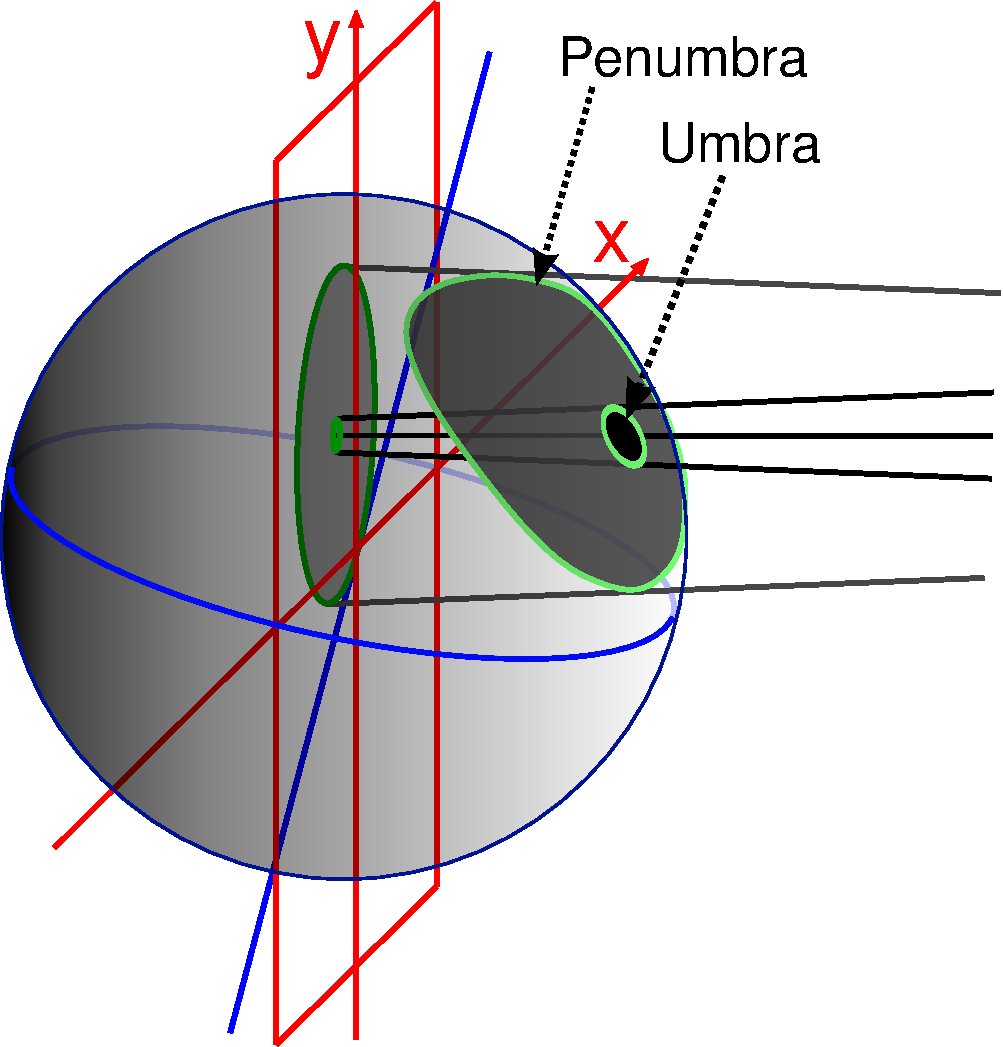
\includegraphics[height=0.74\textheight]{BesselianElementsForTotalEclipse3D-en.pdf}
    \end{column}
    \begin{column}{0.50\textwidth}
      \small
      \begin{itemize}\setlength{\itemsep}{1ex}
        \item Solar eclipse: the Moon's shadow is a \alert{cone} (penumbra, umbra); the fundamental plane
              ($x$, $y$) through the Earth's centre, perpendicular to the shadow axis
        \item Occultation of a star: the star is at infinity, so the asteroid's shadow is a \alert{cylinder}
              of the asteroid's size
        \item Our solver: the plane through \alert{the observer}, the asteroid's light time from the site
              (next slide)
      \end{itemize}
    \end{column}
  \end{columns}
  {\renewcommand{\thefootnote}{}\footnotetext{\tiny Figure: By G.~Pieper, enhanced by User:Iridos, Uploader: Cactus26
   - Own work, CC BY-SA 3.0, \url{https://commons.wikimedia.org/w/index.php?curid=12020673}}}
\end{frame}

% the fundamental plane, oblique 3-D view: z = s (to the star) to the right, y (north) up, x (east) toward the viewer
\begin{frame}{The fundamental plane: geometry}\slideid{FG}
  \centering
  \begin{tikzpicture}[x={(-0.75cm,-0.55cm)}, y={(0cm,1cm)}, z={(1cm,0cm)}, scale=0.84,
                      font=\footnotesize, >={Stealth[length=2.2mm]}]
    % the plane through the observer, perpendicular to the star
    \fill[syzblue!7] (-2,-1.4,0) -- (2.4,-1.4,0) -- (2.4,2.5,0) -- (-2,2.5,0) -- cycle;
    \draw[syzblue!45] (-2,-1.4,0) -- (2.4,-1.4,0) -- (2.4,2.5,0) -- (-2,2.5,0) -- cycle;
    \node[syzblue, anchor=south, align=center] at (-2,2.5,0) {fundamental plane\\through $O$, $\perp\,\uv{s}$};
    % the shadow on the plane: its centre P(t) moves along the track; closest approach to O at t*
    \fill[syzaccent!22] plot[smooth cycle, samples=36, domain=0:350, variable=\t]
         ({0.9+0.45*cos(\t)}, {1.3+0.45*sin(\t)}, 0);
    \draw[->, syzaccent, very thick] (1.97,0.56,0) -- (-0.17,2.04,0);
    \fill[syzaccent] (1.97,0.56,0) circle (1.4pt) node[left, syzaccent] {$P(t_1)$};
    \node[syzaccent, above left=-1pt] at (-0.17,2.04,0) {$P(t_2)$};
    \fill[syzaccent] (0.9,1.3,0) circle (1.6pt) node[left=4pt, syzaccent] {$P(t^{*})$};
    % observer, plane axes, offsets and miss distance
    \draw[densely dotted] (0,0,0) -- (0.9,0,0) node[midway, above left=-2pt] {$\xi$} -- (0.9,1.3,0)
         node[pos=0.4, left] {$\eta$};
    \draw[thick] (0,0,0) -- (0.9,1.3,0) node[pos=0.6, right] {$d_{\min}$};
    \draw[->, thick, syzblue] (0,0,0) -- (1.9,0,0) node[below] {$\uv{x}$ east};
    \draw[->, thick, syzblue] (0,0,0) -- (0,1.5,0) node[right] {$\uv{y}$ north};
    \fill (0,0,0) circle (1.8pt) node[below right=1pt and 0pt] {observer $\vv{O}(t)$};
    % star direction and the star at infinity
    \draw[->, very thick, syzaccent] (0,0,0) -- (0,0,2.0) node[below right=-1pt and 1pt] {$\uv{s}=\uv{z}$};
    \draw[densely dashed, syzaccent] (0,0,2.0) -- (0,0,9.0);
    \node[syzaccent] at (0,0,9.3) {\Large$\star$};
    \node[syzaccent, anchor=north] at (0,0,9.3) {star (at infinity)};
    % asteroid: its motion, and its shadow axis (parallel to s) back to the plane
    \draw[gray, densely dashed, ->] (1.97,0.56,4.8) -- (-0.17,2.04,4.8) node[above] {motion};
    \fill[gray] (1.97,0.56,4.8) circle (1.4pt) node[gray, below] {$\vv{A}(t_1)$};
    \draw[->, syzaccent!80!black, thick] (0.9,1.3,8.2) -- (0.9,1.3,5.05) node[pos=0.4, above] {starlight};
    \draw[syzaccent!80!black, thick, densely dashed] (0.9,1.3,4.8) -- (0.9,1.3,0)
         node[pos=0.55, above] {shadow axis $\parallel \uv{s}$};
    \fill[black!80] (0.9,1.3,4.8) circle (3.2pt) node[below right=1pt] {asteroid $\vv{A}(t^{*}-\tau)$};
    % observer to asteroid, light time from the site
    \draw[->, thick] (0,0,0) -- (0.86,1.24,4.6) node[pos=0.78, below=1pt] {$\vv{\rho}$};
  \end{tikzpicture}\\[0.2ex]
  {\footnotesize $\vv{\rho} = \vv{A}(t-\tau) - \vv{O}(t)$, light time $\tau$ from the site.
   The shadow axis meets the plane at $P = (\xi, \eta) = (\uv{x}\cdot\vv{\rho},\ \uv{y}\cdot\vv{\rho})$;
   closest approach $t^{*}$: $d = |P|$ smallest; hit if $d(t^{*}) < r$ (LT.2, FP.2, CA.1).}
\end{frame}

\begin{frame}{Step 3: the fundamental plane}\slideid{FP}
  \OWN\ Plane through the observer, perpendicular to the star:
  \[
    \uv{z} = \uv{s},\qquad
    \uv{x} = \frac{\uv{e}_3 \times \uv{s}}{|\uv{e}_3 \times \uv{s}|}\ \text{(east)},\qquad
    \uv{y} = \uv{s} \times \uv{x}\ \text{(north)}
    \tag{FP.1}
  \]
  Shadow axis relative to the observer, and the miss distance:
  \[
    \xi(t) = \uv{x}\cdot\vv{\rho}(t),\qquad
    \eta(t) = \uv{y}\cdot\vv{\rho}(t),\qquad
    d(t) = \sqrt{\xi(t)^2 + \eta(t)^2}
    \tag{FP.2}
  \]
  {\small The star is at infinity: its shadow is a cylinder of radius $r$ along $\uv{s}$;
  the observer is inside it when $d(t) < r$.}
\end{frame}

\begin{frame}{Step 4: closest approach and the hit test}\slideid{CA}
  Minimise over an offset from the guess $t_0$ (bracket $T$ from the corridor scan):
  \[
    t^{*} = t_0 + \operatorname*{arg\,min}_{|\Delta t| \le T/2} d(t_0 + \Delta t),
    \qquad d_{\min} = d(t^{*})
    \tag{CA.1}
  \]
  \begin{itemize}
    \item \SC\ \texttt{minimize\_scalar(method='bounded')} (Brent), \texttt{xatol} \SI{1}{ms}; solving for $\Delta t$, not raw ET:
          for $t \approx 8\times10^{8}$\,s the tolerance $\sqrt{\epsilon}\,|t|$ would be $\approx\SI{12}{s}$
    \item Minimum within \SI{1}{s} of the bracket edge: not a real minimum (a neighbour finds it)
  \end{itemize}
  \[
    \text{hit} \iff d_{\min} < r_{\max} + \text{reach}
    \qquad(\text{logged ``in the shadow'': } d_{\min} < r_{\max})
    \tag{CA.2}
  \]
\end{frame}

\begin{frame}{Step 5: observable? and what the observer sees}\slideid{OV}
  \OWN\ Local vertical (geodetic normal) and altitudes at $t^{*}$; \SP\ $\mathsf{R}$ by \texttt{pxform},
  Sun $\uv{s}_\odot$ from the Earth's centre, apparent (``LT+S''):
  \[
    \uv{u} = \mathsf{R}(t^{*})
      \begin{pmatrix}\cos\varphi\cos\lambda\\ \cos\varphi\sin\lambda\\ \sin\varphi\end{pmatrix},
    \quad
    h_\star = \arcsin(\uv{u}\cdot\uv{s}) > h_{\min},
    \quad
    h_\odot = \arcsin(\uv{u}\cdot\uv{s}_\odot) < h_{\odot,\max}
    \tag{OV.1}
  \]
  Speed, chord, duration and drop:
  \begin{gather*}
    v = \frac{\bigl|(\xi,\eta)(t^{*}{+}1\,\mathrm{s}) - (\xi,\eta)(t^{*}{-}1\,\mathrm{s})\bigr|}{2\,\mathrm{s}},
    \qquad
    \ell = 2\sqrt{r^2 - d_{\min}^2},
    \qquad
    \Delta t_{\mathrm{occ}} = \frac{\ell}{v} \tag{OV.2} \\
    \Delta m = 2.5\log_{10}\!\bigl(1 + 10^{0.4(m_{\mathrm{ast}} - m_\star)}\bigr) \tag{OV.3}
  \end{gather*}
  {\small \OWN\ $m_{\mathrm{ast}}$ from $H$, $G$ (IAU H--G system; \SP\ distances, phase angle); kept if $\Delta m \ge 0.1$}
\end{frame}
